\documentclass{standalone}

\usepackage[euler-digits]{eulervm}

\usepackage{tikz}
\tikzset{every node/.style={ellipse,align=center,draw,shade,minimum size=4mm,inner sep=2pt}}
\tikzset{every path/.style={->,>=latex}}
\tikzset{t/.style={rectangle}}
\tikzset{r/.style={top color=red}}
\tikzset{g/.style={top color=green}}
\tikzset{b/.style={top color=blue}}

\usetikzlibrary{shapes}

\begin{document}
    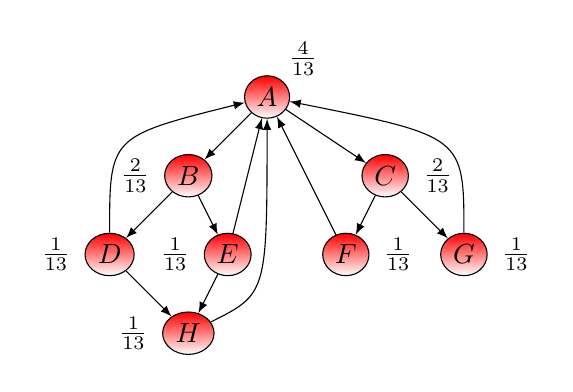
\begin{tikzpicture}[font=\sffamily]
\node[r,label={above right,shade=none:$\frac{4}{13}$}](A) at (0,4) {$A$};
\node[r,label={left,shade=none:$\frac{2}{13}$}](B) at (-1,3) {$B$};
\node[r,label={right,shade=none:$\frac{2}{13}$}](C) at (1.5,3) {$C$};
\node[r,label={left,shade=none:$\frac{1}{13}$}](D) at (-2,2) {$D$};
\node[r,label={left,shade=none:$\frac{1}{13}$}](E) at (-0.5,2) {$E$};
\node[r,label={right,shade=none:$\frac{1}{13}$}](F) at (1,2) {$F$};
\node[r,label={right,shade=none:$\frac{1}{13}$}](G) at (2.5,2) {$G$};
\node[r,label={left,shade=none:$\frac{1}{13}$}](H) at (-1,1) {$H$};


\foreach \s/\t in {A/B,A/C,B/D,B/E,C/F,C/G,D/H,E/H,E/A,F/A}
  \draw (\s) -- (\t);

\draw (H) .. controls (0,1.5) .. (A);
\draw (D) .. controls (-2,3.5) .. (A);
\draw (G) .. controls (2.5,3.5) .. (A);
    \end{tikzpicture}
\end{document}
